\documentclass[11pt]{report}
\usepackage[utf8]{inputenc}
\usepackage[T1]{fontenc}
\usepackage[unicode=true]{hyperref}
\usepackage{lmodern}
\usepackage[french]{babel}

%%% PAGE DIMENSIONS
\usepackage{geometry}
\geometry{a4paper}
\usepackage{graphicx}


%%% PACKAGES
\usepackage{booktabs} % for much better looking tables
\usepackage{array} % for better arrays (eg matrices) in maths
\usepackage{paralist} % very flexible & customisable lists (eg. enumerate/itemize, etc.)
\usepackage{verbatim} % adds environment for commenting out blocks of text & for better verbatim
\usepackage{subfig} % make it possible to include more than one captioned figure/table in a single float
\usepackage{amssymb,amsmath}
\usepackage{xcolor}
\usepackage{sistyle}

\hypersetup{breaklinks=true,
            pdfauthor={Thibault Deutsch (deutsc\_t); Rémy Bernier (bernie\_r); Marc Fresne (fresne\_m); Anthony Belthier (belthi\_a)},
            pdftitle={Rapport de soutenance 1},
            colorlinks=true,
            citecolor=blue,
            urlcolor=blue,
            linkcolor=black,
            pdfborder={0 0 0}}

\setlength{\parskip}{6pt plus 2pt minus 1pt}
\setlength{\emergencystretch}{3em}  % prevent overfull lines

\setcounter{secnumdepth}{3}
\renewcommand{\thesection}{\Roman{section}.}
\renewcommand{\thesubsection}{\arabic{subsection}.}
\renewcommand{\thesubsubsection}{\arabic{subsection}.\arabic{subsection}}

\usepackage{fancyhdr} % This should be set AFTER setting up the page geometry
\pagestyle{fancy}
\fancyhead[L]{Emagine Studio}
\fancyhead[C]{}
\fancyhead[R]{Troma}

\title{Rapport de soutenance 1}
\author{Thibault Deutsch (deutsc\_t) \and Rémy Bernier (bernie\_r) \and Marc Fresne (fresne\_m) \and Anthony Belthier (belthi\_a)}
\date{10 mars 2014}

\begin{document}
\pagenumbering{Roman}

\thispagestyle{empty}
\begin{center}
{\fontsize{30}{32}{\textbf{Troma}}}
\par
\vspace*{0.5cm}
{\fontsize{20}{24}{{\textbf{Rapport de soutenance 1}}}}
\par
{\fontsize{15}{18}{{\textbf{\today}}}}
\end{center}

\vspace*{0.5cm}
\begin{figure}[htbp]
   \begin{center}
      
\includegraphics[scale = 0.05]{eie.png}
   \end{center}
\end{figure}

\vspace*{0.5cm}
\par
\begin{center}
\fontsize{16}{20}
\textbf{Thibault }
\emph{Dethi }
\textbf{Deutsch}
(\emph{deutsc\_t})
\newline
\textbf{Rémy }
\emph{Shadows }
\textbf{Bernier}
(\emph{bernie\_r})
\newline
\textbf{Marc }
\emph{Leshlague }
\textbf{Fresne}
(\emph{fresne\_m})
\newline
\textbf{Anthony }
\emph{AnthonySG }
\textbf{Belthier}
(\emph{belthi\_a})
\newline
\end{center}

\tableofcontents

\newpage
\textbf{{\huge Introduction}} \vspace{7mm}

Ce document est le rapport de la première soutenance et a pour but de présenter le jeu Troma au début de son développement et les prochains objectifs de l’équipe d’Emagine Studio. Pour rappel, le jeu réalisé est un FPS (First-Person Shooter) développé en C\# dont le thème principal est la seconde guerre mondiale. Celui-ci comportera à terme deux modes de jeu : un mode solo, qui sera un contre la montre, et un mode multijoueur.

La répartition des tâches de la première soutenance est présentée dans le tableau ci-dessous.

\begin{figure}[htbp]
\centering
\begin{tabular}{ | c || c | c | c | c | }
\hline Tâches & Thibault & Rémy & Marc & Anthony \\
\hline Modélisation & & & \textcolor{orange}{X} & \\
\hline Moteur graphique & \textcolor{red}{X} & & \textcolor{red}{X} & \\
\hline Moteur physique & & \textcolor{red}{X} & & \textcolor{red}{X} \\
\hline Menu & & \textcolor{red}{X} & & \textcolor{red}{X} \\
\hline Réseau & & & & \\
\hline Gameplay & \textcolor{orange}{X} & \textcolor{orange}{X} & & \\
\hline Audio & & \textcolor{red}{X} & & \textcolor{red}{X} \\
\hline Site web & \textcolor{orange}{X} & \textcolor{orange}{X} & & \\
\hline
\end{tabular}
\caption{Répartition des tâches de la première soutenance}
\end{figure}

\textbf{Légende :}
\begin{itemize}
  \item \textcolor{red}{Rouge} : Commencé
  \item \textcolor{orange}{Orange} : Avancé
\end{itemize}
\vspace*{7mm}

Pour cette soutenance nous souhaitions présenter une carte correspondant au mode entrainement du jeu dans laquelle nous pourrions nous déplacer en vue subjective.

Dans la suite du rapport vous trouverez des explications détaillées à propos du travail fournit par chacun des membres du groupe, des avancées réalisées mais aussi des difficultés rencontrées.
Les conclusions de chaque partie comporteront une liste de prochains objectifs à remplir.

\newpage
\section{Modélisation}

\subsection{La conception}

Avant de commencer la modélisation des différents modèles du jeu il a d’abord fallu réaliser un schéma de la carte pour connaitre leur disposition, dimension mais aussi envisager les différents éléments constituants l’environnement.

Nous avons commencé par choisir le cadre du décor : une petite ferme avec une tranchée établit dans son champ.

Cependant un peu plus tard, après avoir implémenté le terrain, nous nous sommes rendus compte que la disposition que nous avions choisis n’était pas des plus judicieuse puisqu’elle réduisait considérablement la taille du parcours que le joueur devra suivre. En effet la carte dont nous disposons est de forme carrée et d’une dimension plutôt réduite. Nous avons donc élaboré une nouvelle carte ressemblant beaucoup à la première mais permettant d’occuper l’espace de façon plus intéressante.

\subsection{La modélisation}

Une fois que nous avions choisis quels éléments devaient être modélisés, Marc a pu commencer à réaliser les modèles constituant le décor. Deux logiciels ont été utilisés, Blender pour la modélisation, Gimp pour les textures.

Les bâtiments et les éléments de décor tels que les barrières ont été réalisé en se basant sur des formes géométriques simples : cubes, pyramides, triangles, cylindres. L’arme a été réalisé en utilisant un blueprint en arrière-plan afin de facilité la reproduction.

\begin{quote}
``Le terme blueprint désigne, en anglais, un plan détaillé, ce que l'on appelle en dessin technique un dessin de définition. Le terme, signifiant littéralement « impression en bleu », provient d'un procédé d'imprimerie, la cyanotypie.'', \emph{Wikipédia}
\end{quote}

\begin{figure}[htbp]
\centering
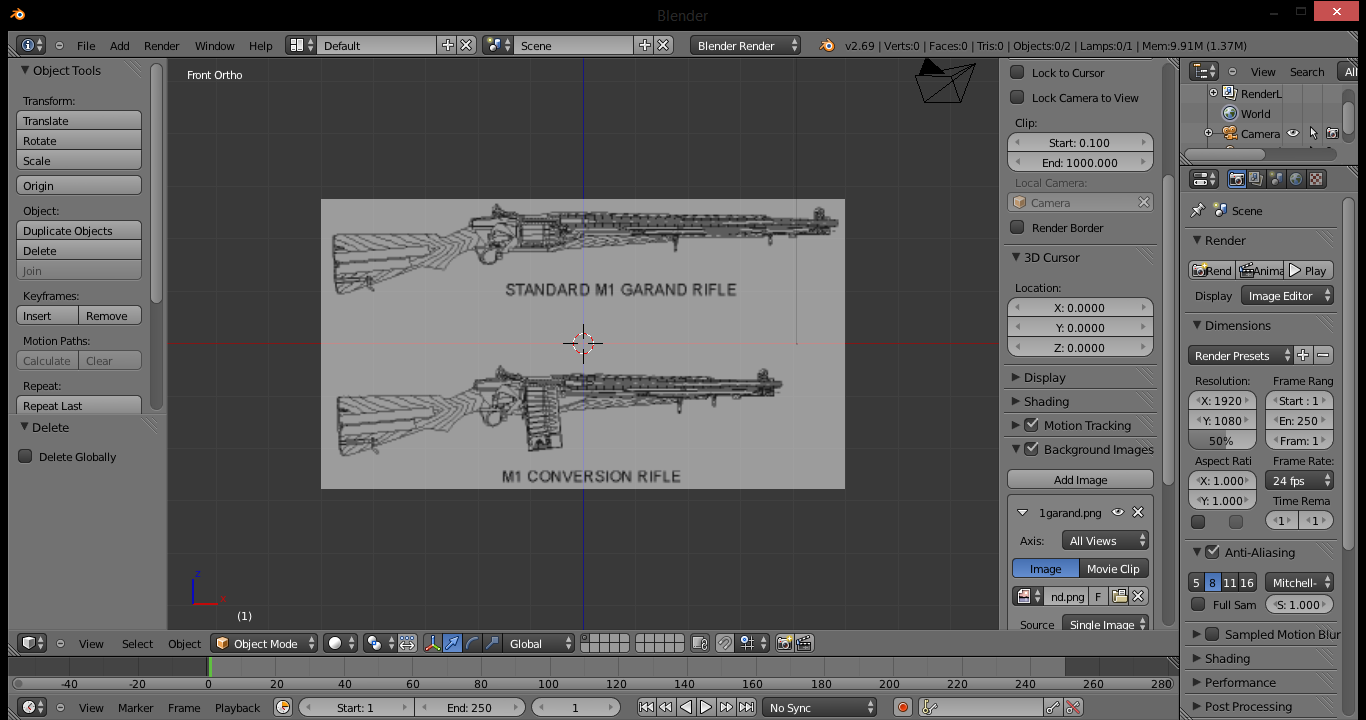
\includegraphics[scale=0.25]{blueprint.png}
\caption{Blueprint sous Blender}
\end{figure}

Les textures des objets 3D utilisent la technique d’UV-Mapping. Celle-ci est une méthode de plaquage de texture qui consiste à déplier l'objet 3D sur une surface plane. Autrement dit on créé le patron de l'objet 3D. On applique alors les textures sur le patron ce qui génèrera une nouvelle image comportant l'ensemble des textures disposées en fonction de la forme du patron. Cette image sera alors déformée, suivant les lignes de découpe du patron, pour être appliquée sur l'objet.

Les modèles ont ensuite été exporté au format FBX pour pouvoir être importé sur XNA.

\subsection{Pour la prochaine soutenance}

Pour la prochaine soutenance, Marc devra réaliser des animations sous Blender qu'il nous faudra ensuite importer et gérer sous XNA. Il faudra aussi réaliser un personnage 3D. En effet celui-ci nous sera utile pour le mode multijoueur. Des améliorations seront également portés sur la carte afin de rendre le jeu plus réaliste et l'adapter aux différents modes de jeu.

\newpage
\section{Moteur graphique}

\subsection{Création du terrain}

Au moment de la conception du terrain, nous avions décidé que celui-ci contiendrait une tranchée. Pour cela il fallait que l'on soit capable d'afficher un sol ayant du relief. Thibault a donc utilisé la technique de l'Heightmap. Cette technique nous permet de créer facilement du relief à partir d'une simple image, de même dimension que le terrain, en se basant uniquement sur le niveau de gris de chaque pixel. On rappel que le niveau de gris correspond à la moyenne des composantes d'un pixel : \( \dfrac{R + G + B}{3} \). 

\begin{figure}[htbp]
\centering
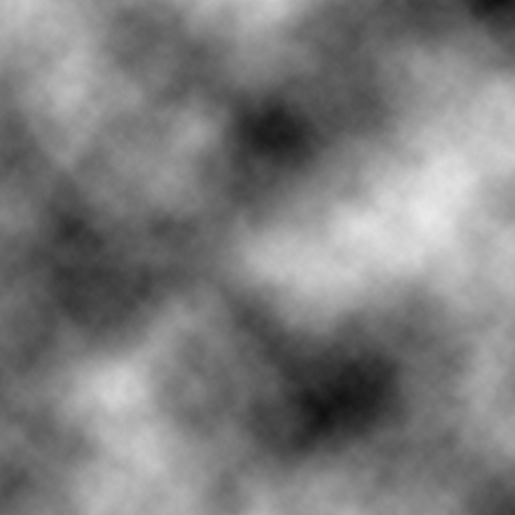
\includegraphics[scale=0.6]{heightmap-texture.png}
\caption{Image en niveau de gris qui peut être utilisée pour l'Heightmap}
\label{fig-heightmap-texture}
\end{figure}

A partir de là, on applique une formule mathématique qui fait le lien entre la hauteur maximale de la carte \( y_{max} \) voulue et le niveau de gris de chaque pixel, noté ici \( \beta \).

\[
y = \dfrac{\left(\dfrac{\beta}{255}\right) - min}{max - min} \times y_{max}
\]

Les valeurs \( min \) et \( max \) permettent d'avoir pour hauteur minimale zéro et pour hauteur maximale \( y_{max} \) quelle que soit l'image utilisée pour le rendu.

\begin{figure}[htbp]
\centering
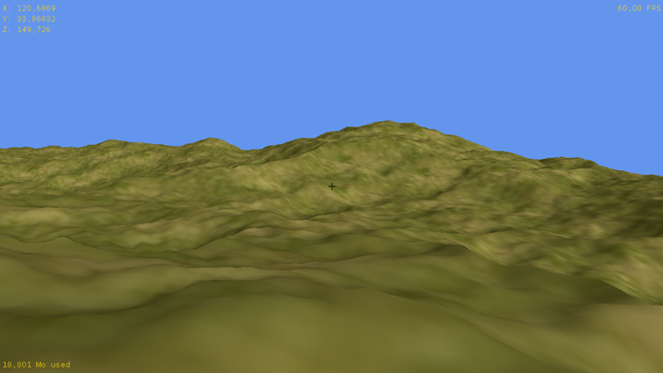
\includegraphics[scale=1]{heightmap-rendu.png}
\caption{Capture d'écran du rendu Heightmap à partir de la fig. \ref{fig-heightmap-texture}}
\end{figure}

Une fois que l'on connait l'ensemble des valeurs \( y \), on applique celles-ci au terrain afin de le déformer.

\subsection{L’importation des fichiers FBX et l’affichage sous XNA}

Pour gérer l'importation et l’affichage nous nous servons basiquement du Content Pipeline d’XNA.

Une fois les modèles réalisés nous avons été confronté à plusieurs problèmes : la taille des modèles, leur orientation, et l’affichage de toutes les faces. Par exemple les modèles étaient trop grands ou alors certaines faces ne s’affichaient pas. De plus tous les modèles apparaissaient retournés de \ang{90} selon l'axe X.

Les problèmes ont été résolus assez rapidement après quelques recherches.

La mauvaise orientation des modèles est due à l'utilisation de repère différent par XNA et Blender. En effet XNA utilise un repère dit main droite. Blender utilise le même repère mais en inversent l'axe Y et Z.

\begin{figure}[htbp]
\centering
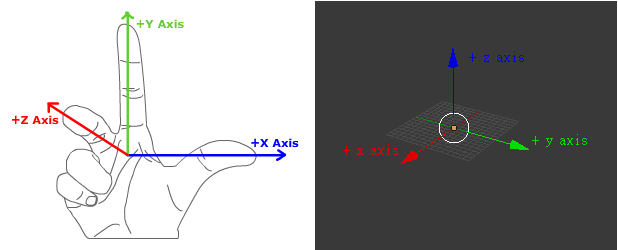
\includegraphics[scale=0.6]{repere.png}
\caption{Repère main droite et repère Blender}
\end{figure}

Concernant l’échelle des objets, une unité Blender correspond exactement à une unité XNA. Il fallait donc juste respecter une échelle sur Blender pour résoudre les problèmes de proportion.

Enfin, les faces cachées étaient dues à une mauvaise modélisation. En effet, chaque objet 3D est composé uniquement de triangle. Chaque triangle est caractérisé par les trois vertex le composant ainsi que le sens de construction du triangle. En effet, afin d'optimiser le rendu 3D, les moteurs graphiques n'affichent par défaut que les faces respectant un même sens de construction. Ce principe permet de ne pas afficher les faces qui sont cachées par un objet 3D. Lors de la création de modèle 3D, la suppression et l'ajout de vertex peuvent provoquer un changement de sens de construction de certain triangle. Heureusement, il est assez facile de corriger ce problème avec Blender.

\begin{figure}[htbp]
\centering
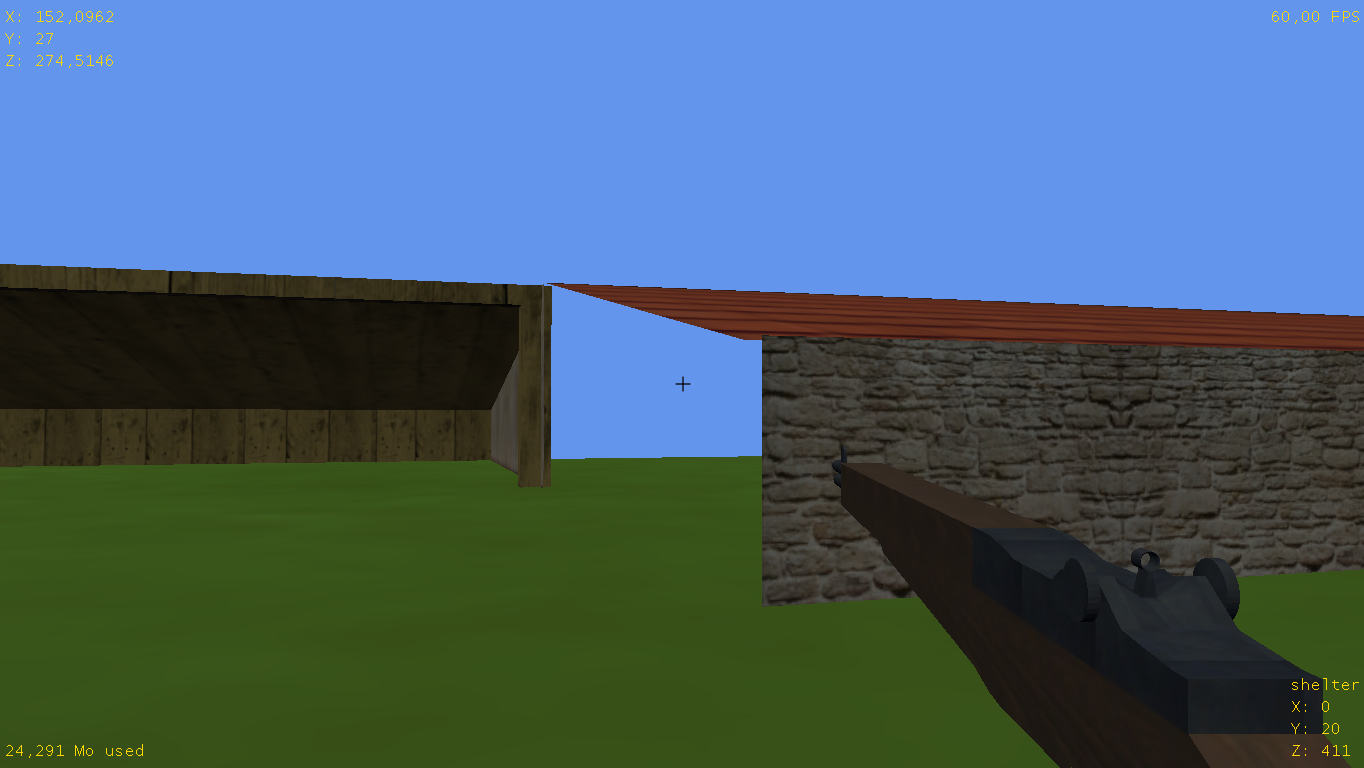
\includegraphics[scale=0.25]{bug-affichage.png}
\caption{Exemple d'un bug d'affichage de certaines faces}
\end{figure}

\subsection{Pour la prochaine soutenance}

Pour la prochaine soutenance, Thibault et Marc réaliserons un skydome afin d'avoir un ciel texturé qui ne sera donc plus monochrome. Ils s'occuperont également de gérer la lumière pour l'ensemble des objets de la map. En effet, actuellement seul le terrain bénéficie d'une lumière diffuse en plus de la lumière ambiante générale.

De plus, la gestion des animations devra être implémentée.

\newpage
\section{Moteur physique}

\subsection{Force gravitationnelle}

La première fonction de notre moteur physique est la fonction gravité. Celle-ci nous permet d'appliquer à n'importe quel objet de notre environnement virtuel une force de gravité semblable à la force gravitationnelle de la terre.

C'est grâce à celle-ci que le joueur peut sauter de manière réaliste.

\subsection{Pour la prochaine soutenance}

Notre nouvel objectif pour le moteur physique est la gestion complète des collisions. En effet, cela n'est pas très agréable, ni pratique, de pouvoir passer à travers tous les objets de la map.

Mais avant d'implémenter les collisions, il nous faudra d'abord faire un travail de recherche important afin de trouver la méthode la plus optimale. Moins il y aura de vérification de collisions, plus le jeu sera fluide. 

\newpage
\section{Menu}

\subsection{Menu de démarrage}

Le menu de démarrage est le premier élément chargé au démarrage de notre jeu. Celui-ci permet au joueur de lancer la partie.

Nous le voulions le plus beau possible afin de donner envie au joueur de lancer le jeu.

\begin{figure}[htbp]
\centering
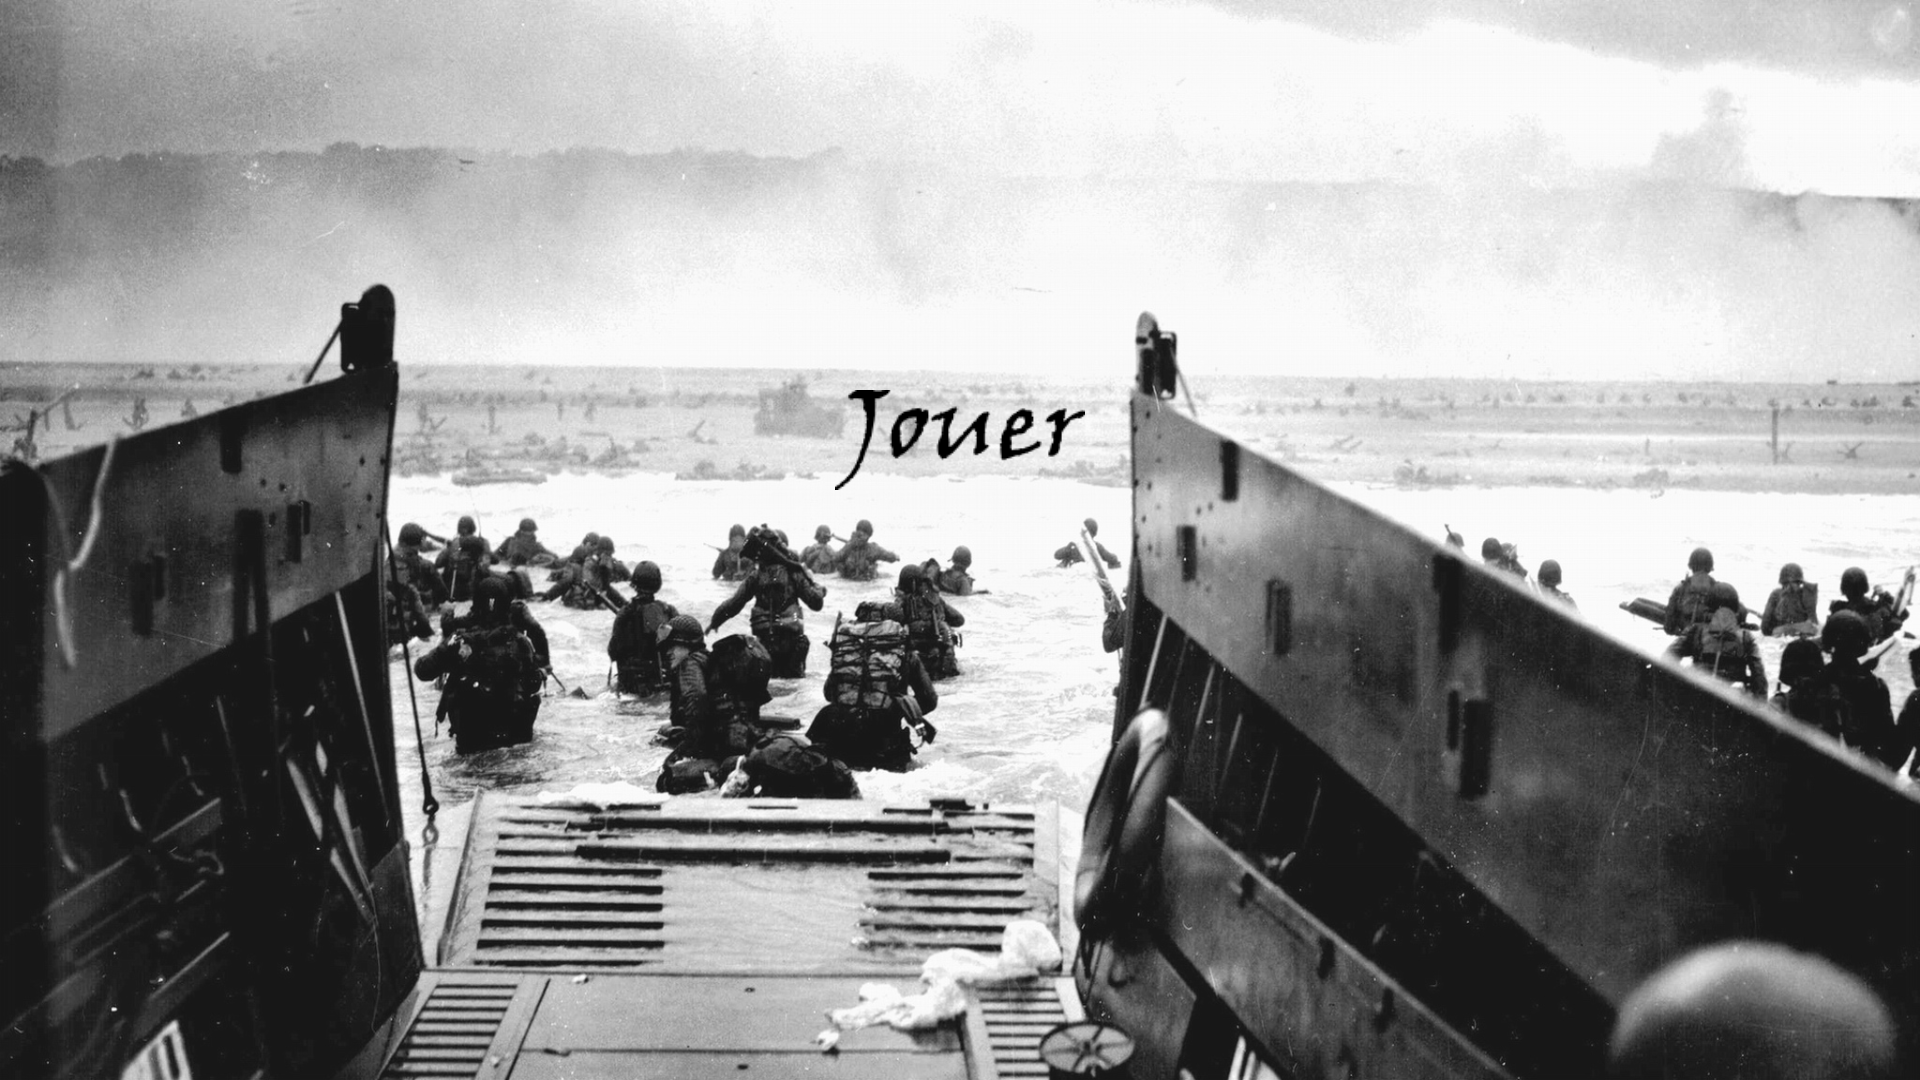
\includegraphics[scale=0.13]{menu-start.png}
\caption{Capture d'écran du menu de démarrage}
\end{figure}

\subsection{Menu de pause}

Le menu de pause, qu'en à lui, permet au joueur de mettre en pause sa partie ou bien de quitter le jeu.

Lors d'une partie, le joueur peut appeler le menu de pause en appuyant sur la touche P de son clavier ou sur la touche START de sa manette Xbox 360.

\begin{figure}[htbp]
\centering
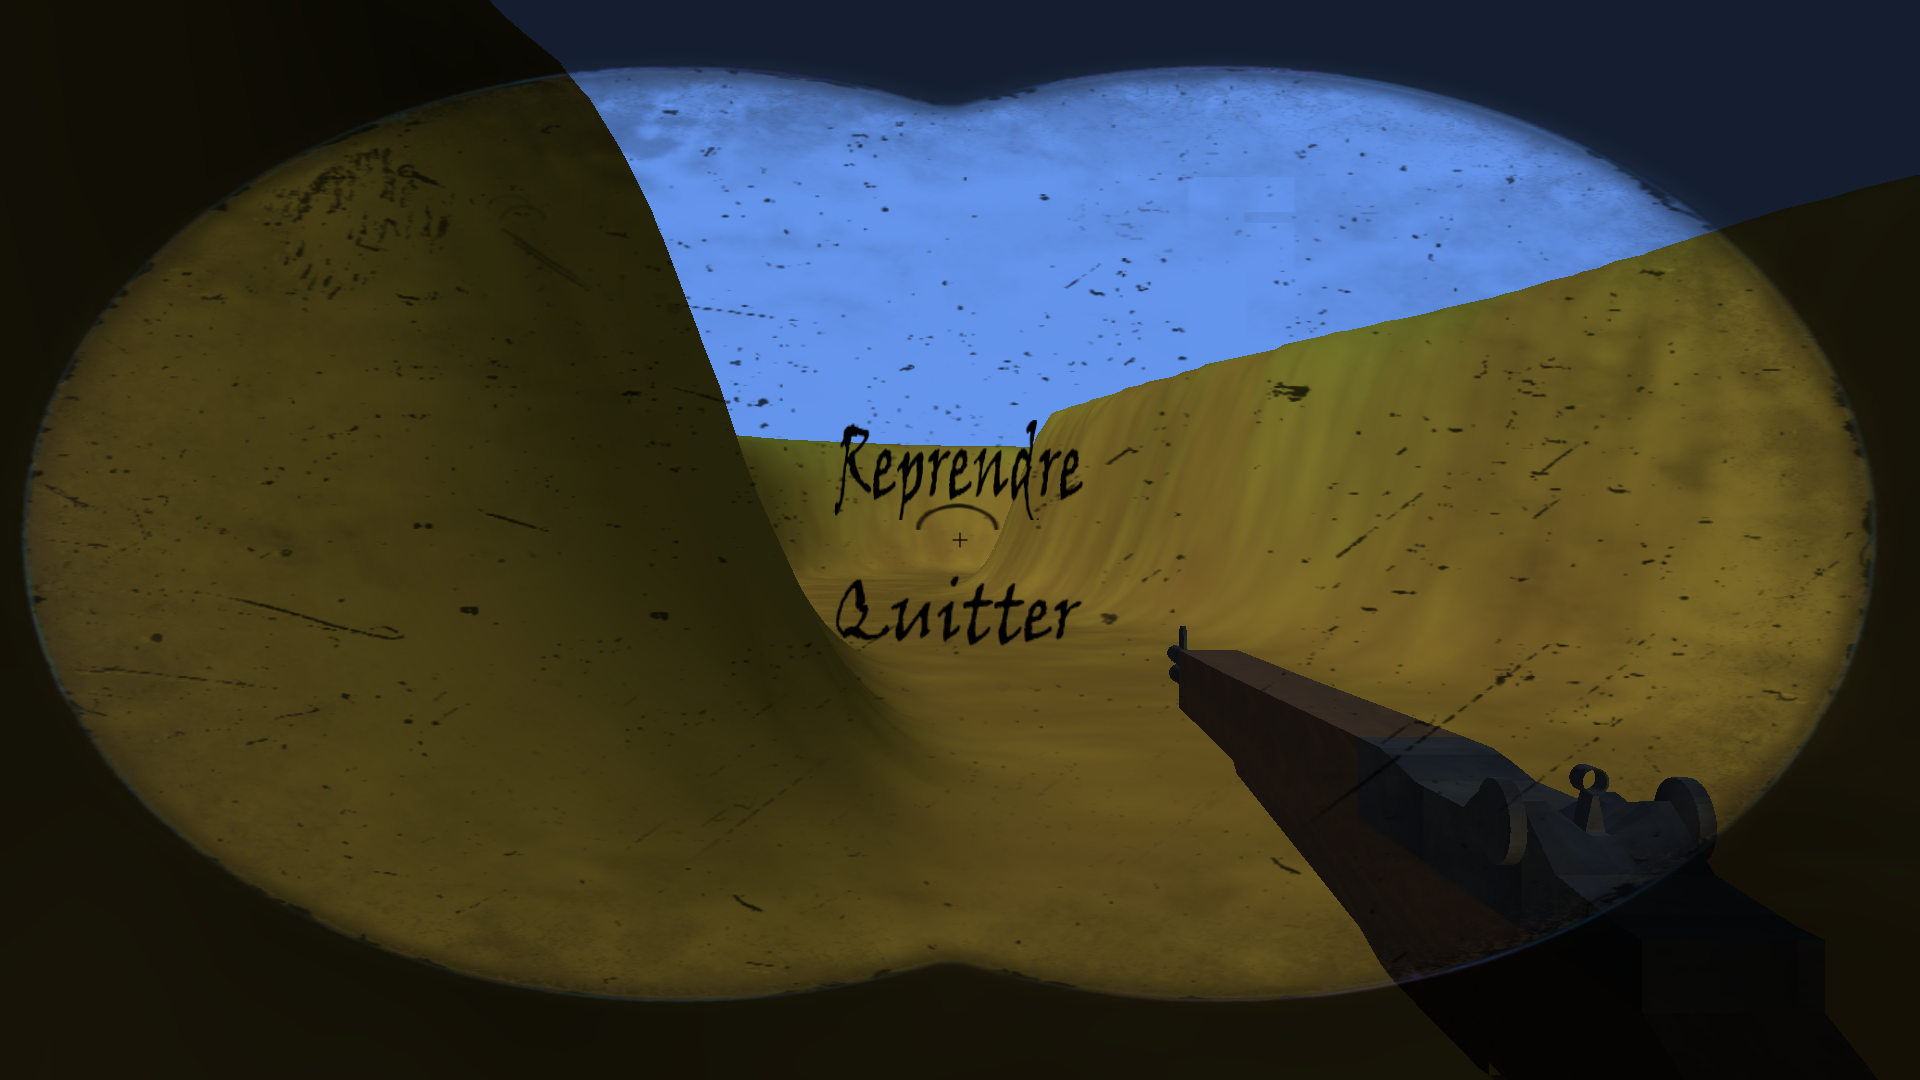
\includegraphics[scale=0.13]{menu-pause.png}
\caption{Capture d'écran du menu de pause}
\end{figure}

\subsection{Pour la prochaine soutenance}

Pour la prochaine soutenance, nous serons capable de nous déplacer dans le menu en utilisant la manette Xbox 360. Pour cela, un important travail de restructuration du code devra être effectué.

Les deux menus auront également des boutons supplémentaires, tel que le bouton QUITTER dans le menu de démarrage.

Et pour finir, Rémy et Anthony commenceront à coder différentes options. Mais celles-ci ne seront pas encore complètement opérationnelles.

\newpage
\section{Réseau}

Pour cette première soutenance, le réseau n'a pas été commencé comme l'indique notre planning. Pour la deuxième soutenance, le réseau et le mode multijoueur auront été commencé mais nous ne pensons pas que ceux-ci seront déjà opérationnels. Nous nous fixons principalement l'objectif d'entamer l'intégration du réseau dans notre structure de code.

\begin{figure}[htbp]
\centering
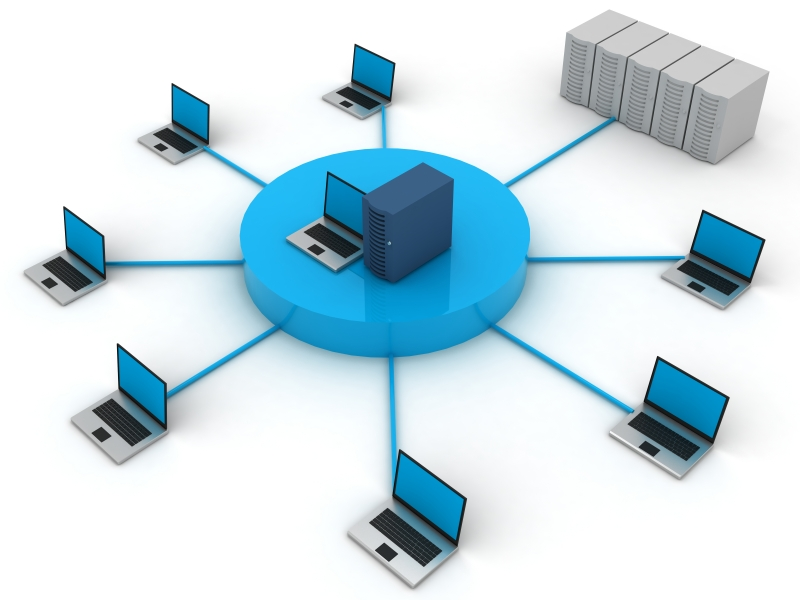
\includegraphics[scale=0.4]{reseau.jpg}
\caption{Schéma d'un réseau centralisé}
\end{figure}

\newpage
\section{Gameplay}

\subsection{Les mouvements du personnage}

Durant cette première période, Thibault et Rémy se sont principalement intéressés aux mouvements du personnage. En effet cela constitue l'ensemble d'éléments le plus basique mais aussi le plus important dans un FPS.

Le personnage peut se déplacer à partir des touches Z, Q, D, S qui représentent respectivement avancer, gauche, droite et reculer. Les touches marchent par paire : Z et S, Q et D. C'est à dire que si vous appuyez sur les deux touches d'une paire en même temps le mouvement s'annule. En effet il est difficile d'aller à droite tout en allant à gauche. Il est également intéressant de noter que nous gérons les mouvements en diagonales. Lors d'un mouvement, le maintien de la touche Z (avancer) et de la touche SHIFT gauche permet de courir.

Le joueur peut également déplacer la souris afin de changer l'angle de la caméra. Pour se faire, nous calculons à chaque fois la différence entre la position d'origine et la nouvelle position du curseur de la souris. Nous appliquons alors un coefficient à cette différence afin d'amplifier le mouvement.

Deux autres mouvements ont été intégré au personnage : s'accroupir et sauter. Ils sont respectivement représentés sur le clavier par les touches CTRL gauche et ESPACE. Le saut a été conçu dans le cadre du moteur physique et donc de la force gravitationnelle.

Enfin pour terminer cette partie, nous avons fait le choix de commencer l'intégration des manettes de jeu. Ainsi le jeu peut d'ores et déjà être entièrement joué avec la manette Xbox 360.

\subsection{Armement}

Notre personnage est un soldat de la seconde guerre mondiale. Il lui faut donc pouvoir se défendre. Afin de réaliser cette tâche, Thibault et Rémy se sont tout d'abord intéressés aux éléments communs de chaque arme, à savoir tirer et recharger. Il a donc fallu intégrer ces différentes actions au niveau du personnage. Comme dans la plupart des FPS, le tir s'effectue avec le bouton gauche de la souris et le rechargement de l'arme avec la touche R.

Il a ensuite fallu intégrer des armes. Pour l'instant une seule est disponible dans le jeu : le M1 Garand. En effet pour chaque arme, un travail important doit être réalisé. Il nous faut d'abord le modèle que Marc réalise en se basant sur des images de l'arme. Ensuite Rémy et Anthony doivent s'occuper de chercher ou réaliser des effets sonores le plus réaliste possible. Et enfin nous pouvons intégrer le tout ensemble. 

Nous avons choisi un processus aussi long pour une seule raison : respecter le contexte historique. Nous essayons au maximum de coller à la réalité. Chaque création d'une arme passe en tout premier lieu par une recherche internet.

\subsubsection*{M1 Garand}

Le Garand M1 est le premier fusil semi-automatique de l'armée américaine. Il possède une cadence de tir de 30 coups/min et son chargeur à une capacité 8 cartouches.

\begin{figure}[htbp]
\centering
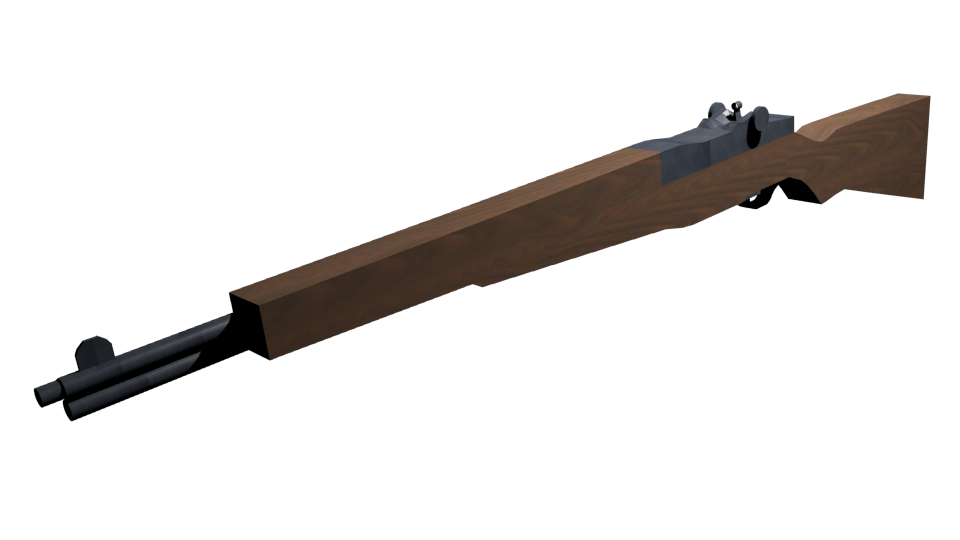
\includegraphics[scale=0.55]{m1-garand.png}
\caption{Modélisation du M1 Garand}
\end{figure}

\subsection{Pour la prochaine soutenance}

Les futurs développements porteront sur l'interface du jeu et la gestion du score. En effet il serait intéressant de pouvoir visualiser le nom de l'arme actuellement utilisée et le nombre de munitions restantes.

De plus nous devrons implémenter le mode d'entrainement de notre jeu. Pour cela une gestion du score devra être réalisée et maintenue tout le long du développement. Notre jeu ne ressemblera donc plus à simple mouvement libre du personnage mais à un réel mode de jeu.


\newpage
\section{Audio}

\subsection{Les effets sonores}

Dans un jeu vidéo, les effets sonores sont aussi importants que le rendu visuel. En effet pour pouvoir s'immerger dans le contexte audio, notre cerveau a besoin d'un retour auditif de ces actions.

Pour cette première soutenance, Rémy et Anthony se sont chargés d'implémenter les différents effets sonores du M1 Garand. Pour cela, ils ont commencé par chercher pendant de nombreuses heures sur internet les sons idéaux. Ils ont finalement trouvé leur bonheur sur le site \url{http://www.freesound.org/}. Il s'agit d'une banque de sons libres et gratuits.

Ainsi le M1 Garand possède un son pour chacun de ses états : tirer, recharger et chargeur vide !

\subsection{La musique de fond}

Rémy s'est également occupé de la musique de fond. Celle-ci n'apparait que dans les menus : le menu de démarrage et le menu de pause. La musique tourne en boucle et se coupe dès que l'on quitte les menus.

\subsection{Pour la prochaine soutenance}

Pour la soutenance 2, Rémy et Anthony rajouteront différents effets sonores tel que les bruits de pas.

\newpage
\section{Site web}

\subsection{La conception du design}

Pour la conception du site web, un petit challenge entre Thibault et Rémy a été organisé. Ils devaient concevoir de leur côté un design complet du site. Le gagnant sera alors celui dont le design plaira le plus au reste de l'équipe et à un petit groupe d'amis.

Ils ont alors chacun conçu des design sur papier puis réalisé une première ébauche du site. Une seule limitation leur était imposée : le site devait être ``responsive desgin''. C'est à dire qu'il doit s'adapter à toutes les tailles d'écrans : ordinateur de bureau, ordinateur portable, tablette et smartphone.

Il n'y a eu finalement aucun gagnant. Thibault et Rémy ont préféré fusionner leur deux visions différentes pour créer le design actuel de notre site web.

Le site a été conçu avec Foundation, un framework HTML/CSS/Javascript qui permet de concevoir très rapidement des sites internet avec de nombreuses fonctionnalités. Mais le grand intérêt de ce type de framework est qu'ils sont pensés pour être ``responsive design'' et qu'ils s'affichent à l'identique sur l'ensemble des navigateurs internet. Un avantage de Foundation par rapport à ces concurrents est une plus grande facilité de personnalisation du design de base. Tout est pensé pour obliger le développeur à y intégrer sa propre vision.

\begin{figure}[htbp]
\centering
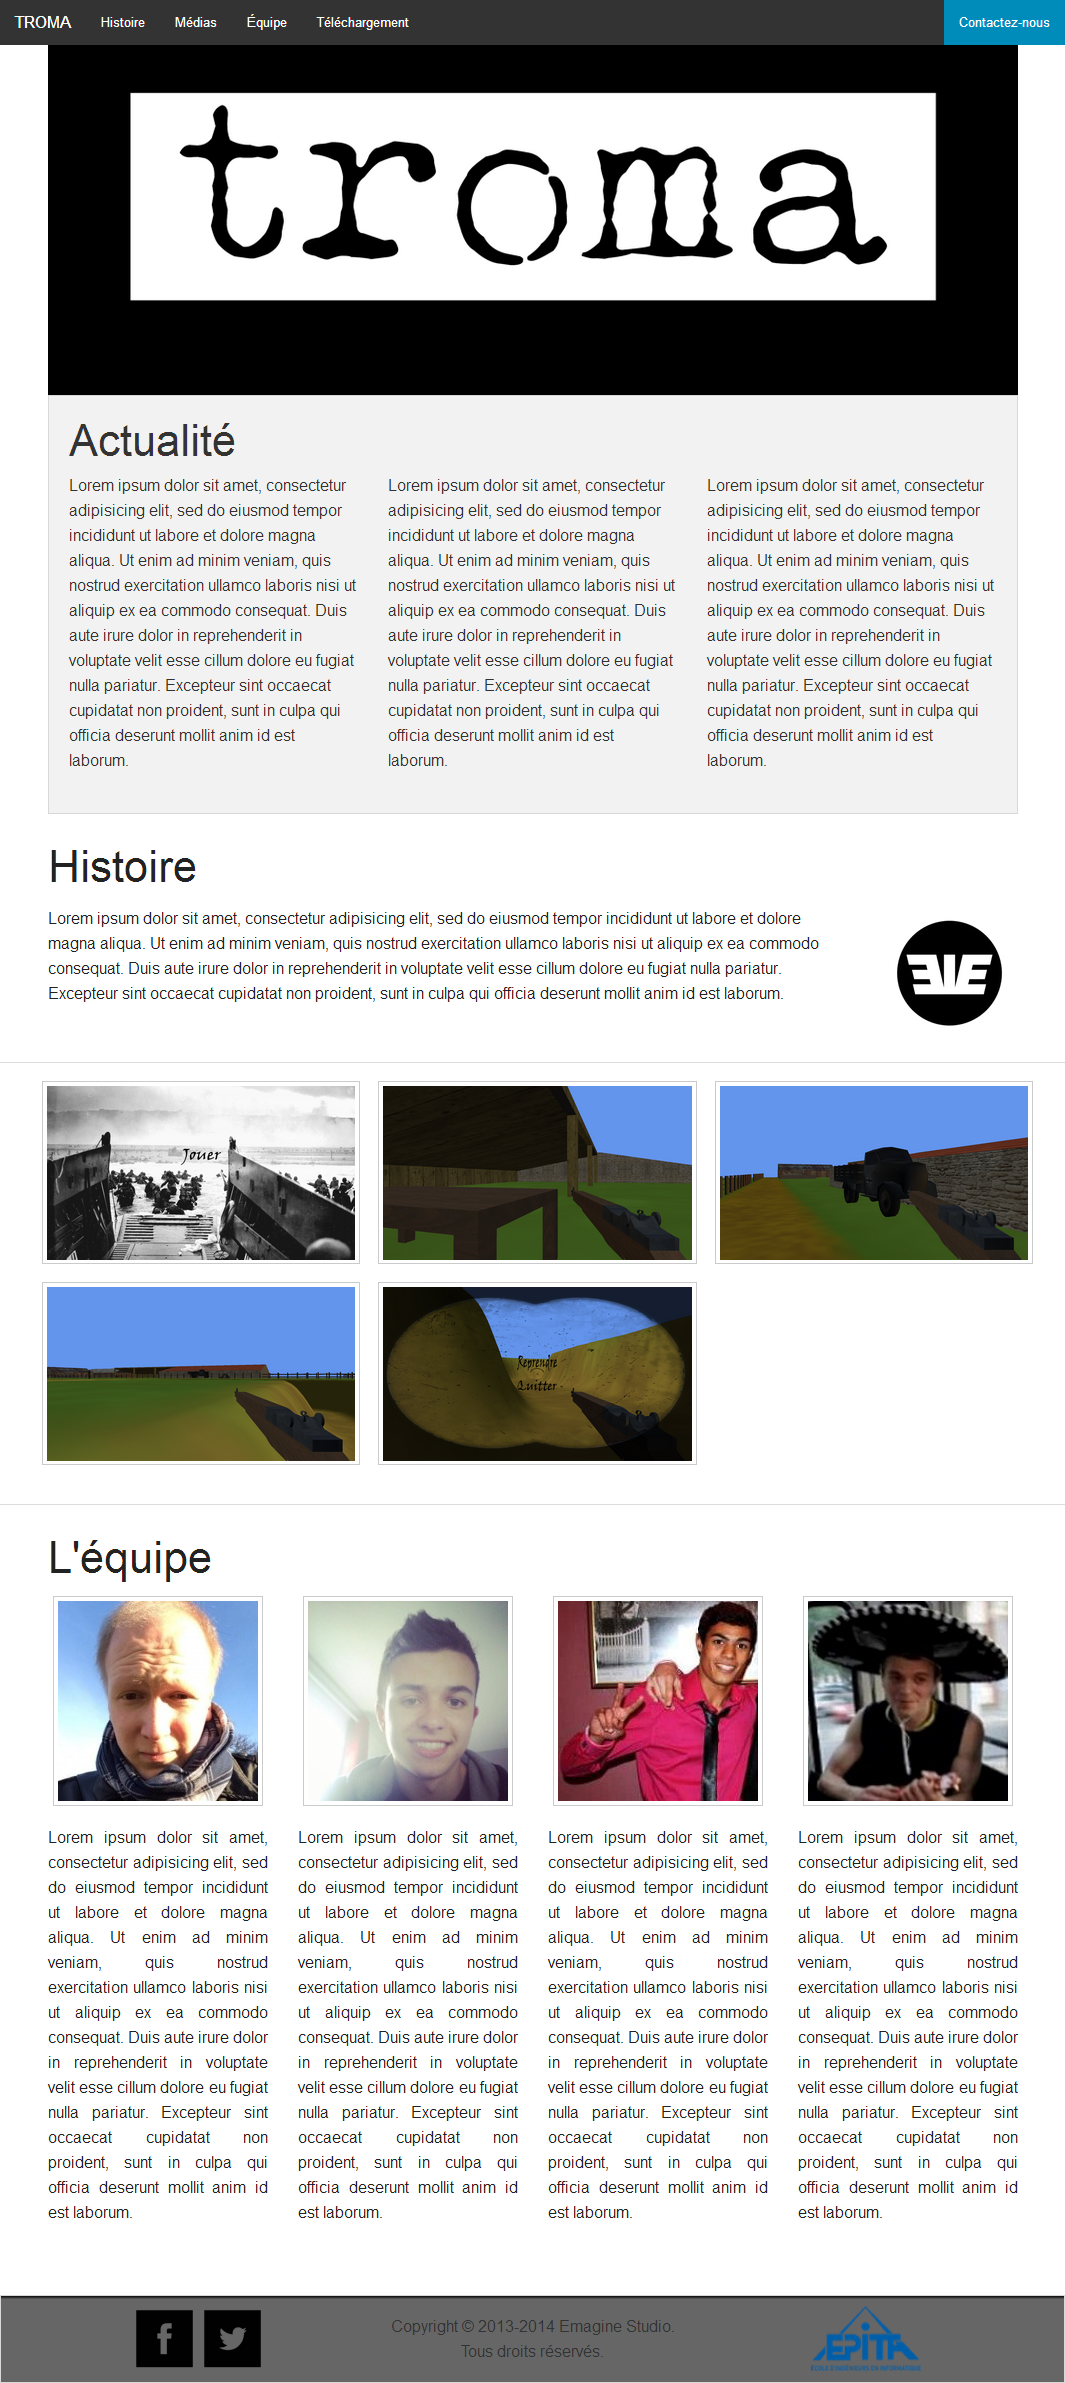
\includegraphics[scale=0.23]{siteweb.png}
\caption{Maquette finale du design du site web}
\end{figure}

\subsection{Contenu et accès au site internet}

Le site web comporte actuellement :

\begin{itemize}
  \item l’histoire du personnage principal dans le jeu, afin de donner envie au visiteur de télécharger et de jouer à notre jeu.
  \item un ensemble de capture d'écran régulièrement actualisé
  \item la présentation de notre équipe, avec des photos et de petites descriptions.
  \item la progression actuelle de la conception de notre jeu
  \item une partie téléchargement
  \item un ensemble d'information pour nous contacter par mail ou sur les réseaux sociaux.
\end{itemize}

Notre site internet est accessible à l'adresse \url{http://www.troma.eu/}. A partir de celui-ci vous pouvez avoir accès aux réseaux sociaux sur lesquels nous essayons d'être régulièrement actif !

\subsection{Pour la prochaine soutenance}

D'ici la deuxième soutenance, le site web possèdera un blog pour pouvoir communiquer sur les actualités autour de notre jeu, ainsi que des améliorations par-ci par-là de notre design.

\newpage
\textbf{{\huge Conclusion}} \vspace{7mm}

Ces premières semaines de projet auront été très motivantes. Toutes les difficultés que nous avons rencontrées ont été surmonté. De plus nous avons respecté notre planning, voir sur certaines parties nous avons pris une légère avance. Nous espérons garder cette avance pour pouvoir surmonter toutes les difficultés qui nous attendent. En effet, ce n'est que le début de l'aventure et la difficulté ne fera qu'augmenter au cours du projet.

\begin{figure}[htbp]
\centering
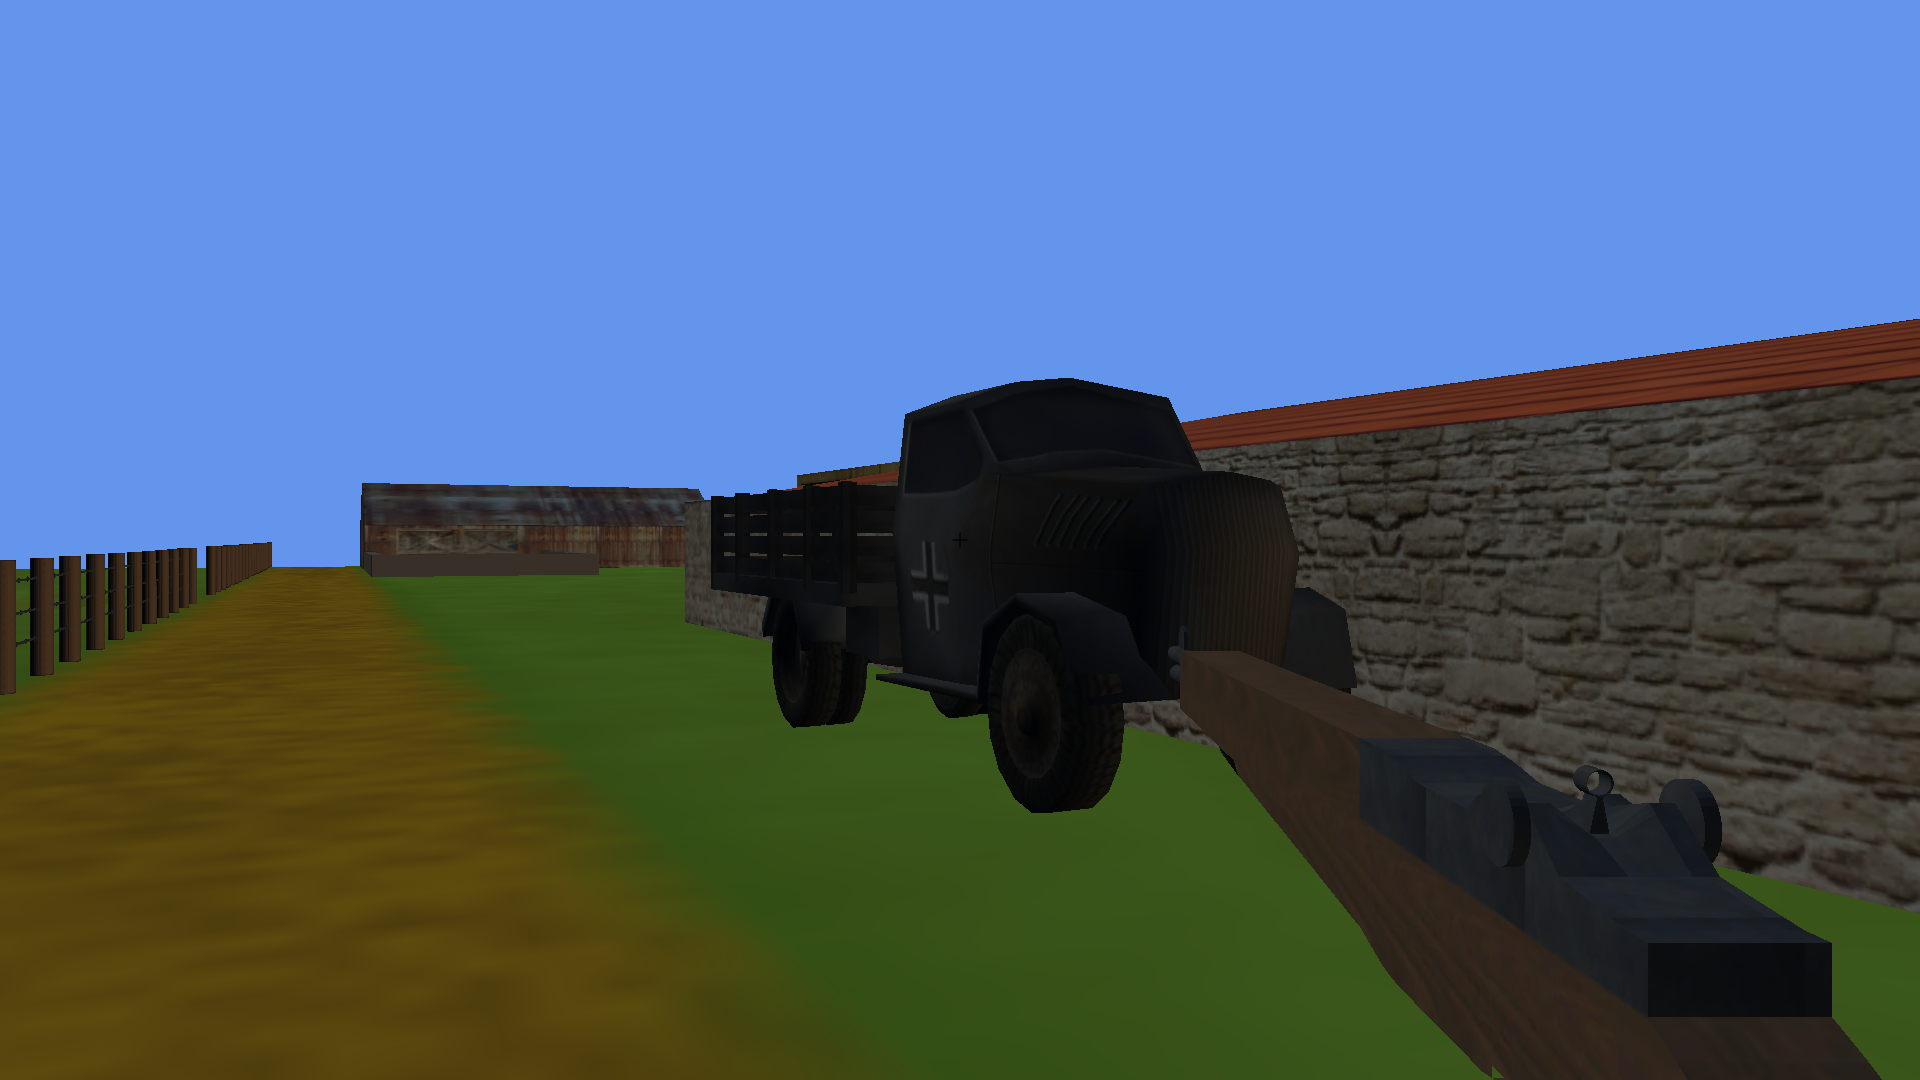
\includegraphics[scale=0.18]{resultat-1.png}
\caption{Capture d'écran du jeu pour la première soutenance}
\end{figure}

Nous sommes très fiers du rendu de notre jeu pour cette première soutenance. Espérons que la motivation restera avec nous !

Enfin pour finir avec quelques statistiques intéressantes, notre jeu est composé actuellement d'un peu moins de 200 fichiers, pour un total de 9579 lignes de code.

\newpage
\listoffigures 
 
\end{document}